% Capturas originales de la ejecución personal del 21/11/2026.
% Respaldo sin numeración: no añade tiempo obligatorio a la exposición.
\begin{frame}[plain,noframenumbering,label=gs-evidencia-general]{Evidencia general: dos ventas para una unidad}
  \centering
  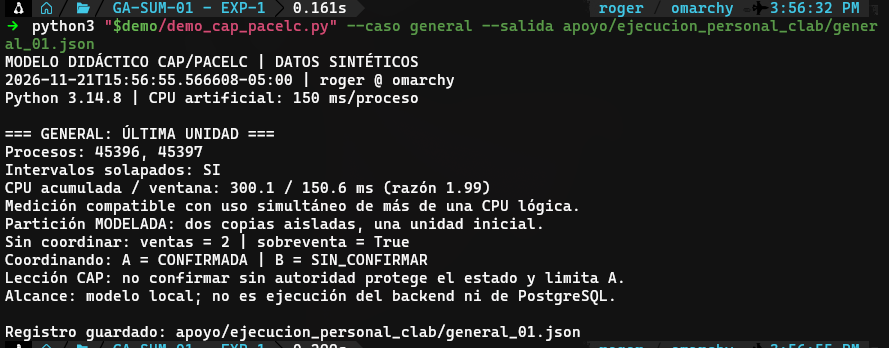
\includegraphics[width=\textwidth,height=0.65\paperheight,keepaspectratio]{evidencias/garcia_sangoquiza/01_cap_general.png}\par
  {\scriptsize Ejecución personal, 21/11/2026. Trabajo CPU artificial:
  300,1 ms acumulados en 150,6 ms. Partición modelada; no se cortó la red.}\par
  \hyperlink{gs-cap}{\beamerreturnbutton{Volver a CAP}}
\end{frame}

\begin{frame}[plain,noframenumbering,label=gs-evidencia-clab]{Evidencia CLAB: consultar no es reservar}
  \centering
  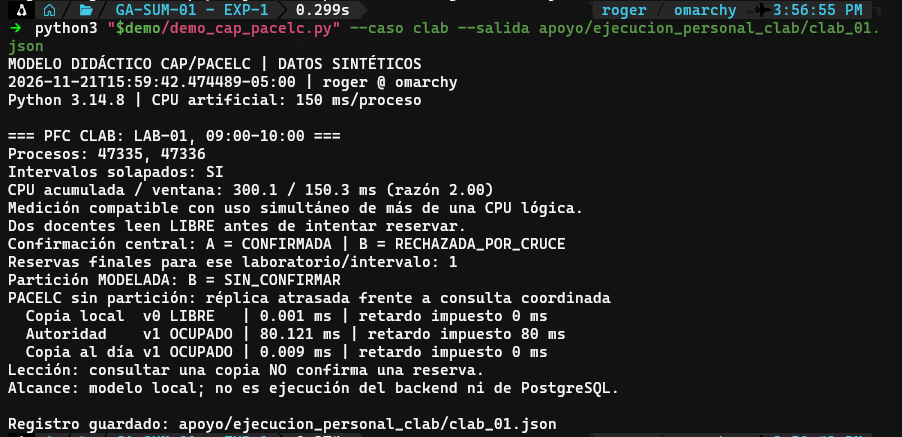
\includegraphics[width=\textwidth,height=0.65\paperheight,keepaspectratio]{evidencias/garcia_sangoquiza/02_clab_cap_pacelc.png}\par
  {\scriptsize Una reserva confirmada. Consulta coordinada: 80,121 ms,
  incluidos 80 ms de espera impuesta. Modelo Python, no backend CLAB.}\par
  \hyperlink{gs-pacelc}{\beamerreturnbutton{Volver a PACELC}}
\end{frame}
